\hypertarget{developers}{\section{Foundation model developers}}
\label{sec:developers}


\begin{table}[htp]
\resizebox{\textwidth}{!}{
\begin{tabular}{ccccccccccc}
\toprule
Name & Flagship & Release & Input & Output & Status & Headquarters & WH1 & WH2 & WH3 & FMF \\
\midrule
\aitwentyone & \jurassic & API & Text & Text & Startup & Tel Aviv, Israel & \xmark & \xmark & \xmark & \xmark \\
\amazon & \titan & API & Text & Text & Big Tech & Seattle, USA & \xmark & \cmark & \xmark & \xmark \\
\anthropic & \claude & API & Text & Text & Startup & San Francisco, USA & \cmark & \cmark & \xmark & \cmark \\
\cohere & \command & API & Text & Text & Startup & Toronto, Canada & \cmark & \xmark & \cmark & \xmark \\
\google & \palm & API & Text & Text & Big Tech & Mountain View, USA & \cmark & \cmark & \xmark & \cmark \\
\huggingface & \bloomz & Open weights, open data & Text & Text & Startup & Brooklyn, USA & \cmark & \xmark & \xmark & \xmark \\
\inflection & \inflectionone & No access (API forthcoming) & Text & Text & Startup & Palo Alto, USA & \xmark & \cmark & \xmark & \xmark \\
\meta & \llama & Open weights & Text & Text & Big Tech & Menlo Park, USA & \xmark & \cmark & \xmark & \xmark \\
\openai & \gptfour & API & Text, Images & Text & Startup & San Francisco, USA & \cmark & \cmark & \xmark & \cmark \\
\stability & \stablediffusion & Open weights, open data & Text & Images & Startup & London, UK & \cmark & \xmark & \cmark & \xmark \\
\bottomrule 
\end{tabular}}

\caption{\textbf{Selected foundation model developers.} 
Information on the \numcompanies selected foundation model developers: the developer name, their flagship model, the release strategy for the model (see \reffig{release-gradient}), the input and output modalities for the model, the developer's status as either Big Tech or Startup, and the developer's headquarters.
We note which of the developers were involved in the White House's initiative for public evaluation of AI systems announced in May 2023 (WH1), voluntary commitments for the management of risks posed by AI announced in July 2023 (WH2), and commitments by additional organizations on the same matters of risks by AI announced in September 2023 (WH3). 
Additionally, we note which of the developers are founding members of the Frontier Model Forum, announced in July 2023.
}
\label{tab:developer-info}
\end{table}

\noindent Transparency initiatives in AI (\eg datasheets and model cards) often introduce frameworks that support machine learning developers in achieving greater transparency in their own work.
In contrast, we proactively assess foundation model developers for their transparency using the \numindicators indicators we specify.
By conducting the assessment ourselves, we sidestep concerns of uneven uptake that have arisen with past transparency initiatives \citep[\eg][]{gebru2018datasheets, mitchell2018modelcards} and provide greater consistency in the scoring of each indicator across developers.
Most importantly, scoring many developers allows for the comparison of their scores, which provides a rich context for how to improve transparency in the foundation model ecosystem.



% Given that we choose to assess the transparency of foundation model developers, we must select the developers to be assessed. 
Efforts like Ecosystem Graphs \citep{bommasani2023ecosystem} and the UK Competition and Markets Authority (CMA) report on the foundation model market\footnote{\url{https://www.gov.uk/government/publications/ai-foundation-models-initial-report}} track the organizations that develop foundation models.
At the time of writing in September 2023, the CMA report documented 160 foundation models (based on data drawn from Ecosystem Graphs) built by more than 50 organizations.\footnote{\url{https://assets.publishing.service.gov.uk/government/uploads/system/uploads/attachment_data/file/1185508/Full_report\_.pdf\#page=22}} 
However, as the CMA report states, a small number of developers control the majority of the market at present \citep{vipra2023concentration}.
Due to this intense level of market concentration, we decided to assess \numcompanies major foundation model developers.  \clearpage

\hypertarget{developer-selection}{\subsection{Selecting developers}}
\label{sec:developer-selection}
We considered a variety of selection criteria in choosing the \numcompanies developers to assess, arriving at the following three principles:
\begin{enumerate}
    \item \textbf{Impact.} We selected developers that have built the most influential foundation models.
    \item \textbf{Diversity.} We selected developers that, when considered collectively, represent many axes of variation in the foundation model ecosystem. For example, developers that release models along different points on the release gradient \cite[\eg open vs. closed,][]{solaiman2023gradient}, build models with different modalities (\eg text-to-text vs. text-to-image), and occupy different positions in the market (\eg startups vs. Big Tech). 
    \item \textbf{Companies.} 
    We selected developers that are established companies as enduring targets for longitudinal improvement. 
    This to some extent parallels current regulatory initiatives that explicitly focus on companies as the target of policy for foundation models.\footnote{See \url{https://www.blumenthal.senate.gov/imo/media/doc/09072023bipartisanaiframework.pdf}.} 
\end{enumerate}
On this basis, we chose 10 companies that all are influential foundation model developers: 
\aitwentyone, \amazon, \anthropic, \cohere, \google, \huggingface, \inflection, \meta, \openai, and \stability.
These \numcompanies provide significant diversity in terms of release strategy (\eg \anthropic, \meta, and \huggingface all release flagship models with different levels of openness; see \Cref{fig:release-gradient}), modality (\eg \cohere, \openai, and \stability all provide different input-output modalities), and market position (\eg \google, \inflection, and \openai occupy different market positions).

Additionally, in parallel to our research, the White House made three announcements involving companies that develop foundation models: a red-teaming exercise announced in May 2023,\footnote{\url{https://www.whitehouse.gov/briefing-room/statements-releases/2023/05/04/fact-sheet-biden-harris-administration-announces-new-actions-to-promote-responsible-ai-innovation-that-protects-americans-rights-and-safety/}} a set of voluntary commitments announced in July 2023,\footnote{\url{https://www.whitehouse.gov/briefing-room/statements-releases/2023/07/21/fact-sheet-biden-harris-administration-secures-voluntary-commitments-from-leading-artificial-intelligence-companies-to-manage-the-risks-posed-by-ai/}} and another set of voluntary commitments announced in September 2023.\footnote{\url{https://www.whitehouse.gov/briefing-room/statements-releases/2023/09/12/fact-sheet-biden-harris-administration-secures-voluntary-commitments-from-eight-additional-artificial-intelligence-companies-to-manage-the-risks-posed-by-ai/}}
% Redteaming - Anthropic, Google, Hugging Face, Microsoft, NVIDIA, OpenAI, and Stability AI (7)
% Commitments 1 - Amazon, Anthropic, Google, Inflection, Meta, Microsoft, and OpenAI (7)
% Commitments 2 - Adobe, Cohere, IBM, Nvidia, Palantir, Salesforce, Scale AI, and Stability (8)
Separately, three of the companies we assess jointly announced the formation of the Frontier Model Forum in July 2023.\footnote{\url{https://blogs.microsoft.com/on-the-issues/2023/07/26/anthropic-google-microsoft-openai-launch-frontier-model-forum/}} 
When taken together, these announcements name 16 companies: Adobe, Amazon, Anthropic, Cohere, Google, Hugging Face, IBM, Inflection, Meta, Microsoft, NVIDIA, OpenAI, Palantir, Salesforce, Scale AI, and Stability AI.
We note that 9 of the 10 companies we selected are within this set of 16 (all but \aitwentyone).


\begin{figure}[t]
\centering
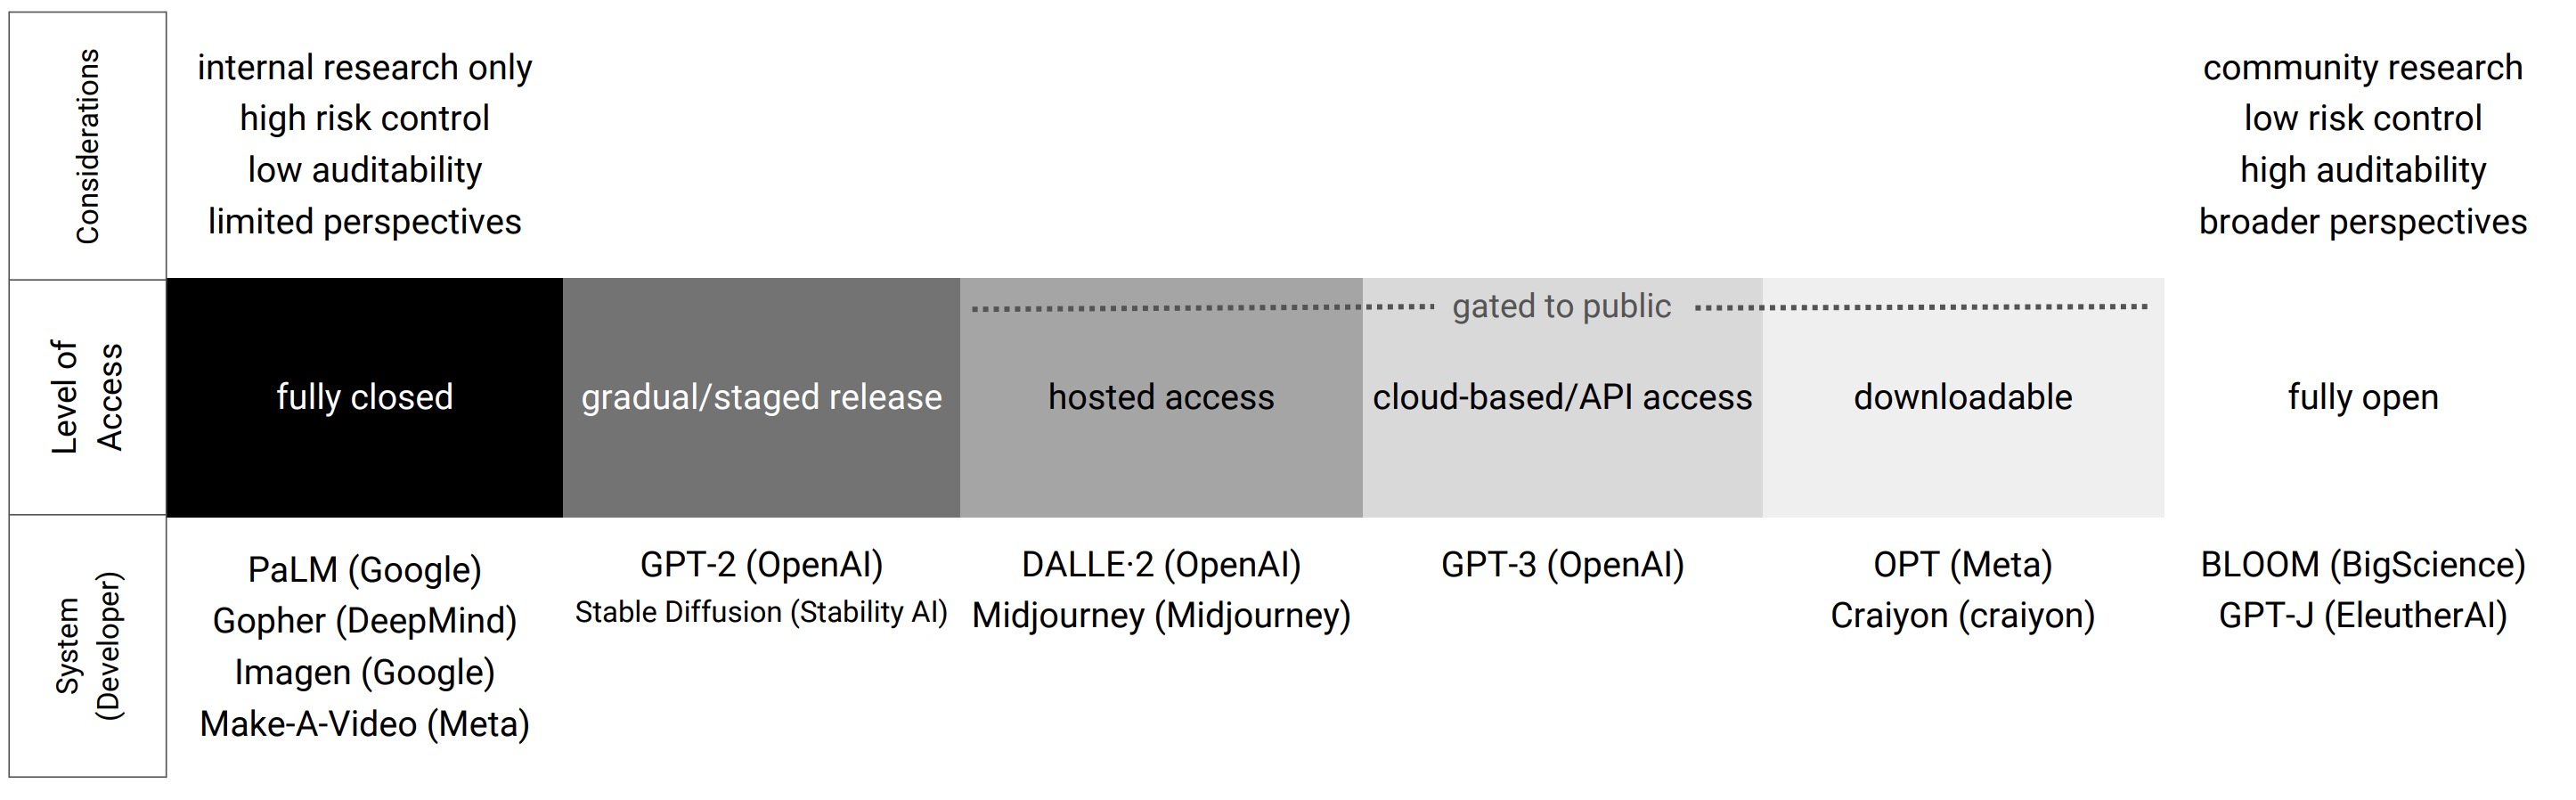
\includegraphics[width=\textwidth]{figures/gradient.jpg}
\caption{\textbf{The gradient of release of foundation models.} 
Foundation models can be fully closed (\eg only used internally within the company, without public release), 
released gradually as their risks and benefits are better understood (\eg via a staged rollout involving initial testers), 
released via a web or app interface (\eg users need to visit a website or join a Discord server to access the model's outputs), 
released via a programmatic API (\eg users can query the model and receive outputs programmatically), 
released via downloadable model weights (\eg users can access and adapt the model), 
or released with the training data alongside downloadable model weights (\ie ostensibly maximal openness). 
For the ten models we consider, one falls under the fully closed category at the time of writing (Inflection-1), though \inflection plans to make it available via an API; six are available via an API (\gptfour, \claude, \palm, \jurassic, \command, \titan); one is downloadable (\llama), and two are released with their model weights as well as underlying training data downloadable (\stablediffusion and \bloomz). 
For simplicity, we at times binarize these distinctions into models with downloadable weights ("open") and models without downloadable weights ("closed").
Image taken with permission from \citet{solaiman2023gradient}.}
\label{fig:release-gradient}
\end{figure}

\paragraph{The gradient of release strategies.}
The strategies for releasing foundation models differ widely (see \reffig{release-gradient}). Some developers release the weights of the model as well as the data used, which allows independent researchers and developers to use the models on their own and investigate the data. For example, EleutherAI released the weights of its Neo-X model \citep{black2022neox} along with The Pile, which Neo-X was trained on \citep{gao2021thepile}.
\meta released the weights to its OPT model \citep{zhang2022opt}, but did not release the associated training data.
For our purposes, we will often refer to any release where model weights are made broadly available as "open," which includes the flagship models of \huggingface, \meta, and \stability.

In contrast, other developers do not release the weights of their flagship model, retaining greater control over who has access to the model and the extent to which it may be used externally (if at all).
The majority of the developers we assess provide a programmatic API to query their flagship model as a black box.
Other developers in the ecosystem do not provide a programmatic API but do allow for some forms of black box access, as Midjourney does for its text-to-image models that it makes available via a Discord server.\footnote{See \url{https://docs.midjourney.com/docs/midjourney-discord}.}
Still other developers provide no external access to their models as is the case for Google's Chinchilla model \citep{hoffmann2022chinchilla} and Meta's Make-A-Video model \citep{singer2022makeavideo}.
For our purposes, we will often refer to any release where model weights are not made externally available as "closed," which includes the flagship models of \aitwentyone, \amazon, \anthropic, \cohere, \google, \inflection, and \openai.

The overall approach to release is informed by a developer's business strategy and perspective on its model's utility and risks. 
In particular, many organizations may adopt different release approaches for different foundation models.
For example, when releasing \gptfour, \openai did not disclose many details about the modeling architecture and training data, citing competition and safety as the two main reasons.\footnote{Interview with \openai's chief scientist and co-founder: \url{https://www.theverge.com/2023/3/15/23640180/openai-gpt-4-launch-closed-research-ilya-sutskever-interview}} 
On the other hand, when releasing the text-to-speech Whisper model \cite{radford2022whisper}, \openai disclosed many details and released the model weights openly.
For other developers, the release decision may directly relate to their purpose for building a foundation model in the first place.
For example, the BigScience collaboration led by \huggingface that led to the BLOOM model \citep{scao2022bloom} was explicitly designed to democratize access to multilingual large language models with capabilities in traditionally underrepresented languages.
As a result, the initiative released model weights and data. \clearpage

\hypertarget{model-selection}{\subsection{Selecting flagship models}}
\label{sec:model-selection}
Almost all major foundation model developers release multiple foundation models over time and, even at the time of writing, many have multiple salient foundation models (often across different modalities).
For example, OpenAI has developed GPT, GPT-2, GPT-3, GPT-4, InstructGPT, WebGPT, Codex, CLIP, DALL-E, DALL-E 2, DALL-E 3, Jukebox, and Whisper among other models.
Given that developers are not guaranteed to provide uniform transparency for each foundation model (\eg OpenAI releases the weights openly for some of these models but not others), we decide to assess developers in relation to their \textit{flagship} foundation model.
By flagship foundation model, we mean the foundation model that is most salient and/or capable from the developer based on our judgment, which is directly informed by the company's public description of the model.
We provide basic information about each of the developers and their flagship model in \reftab{developer-info}.\footnote{For OpenAI, we evaluate GPT-4, which was released in March 2023, not GPT-4V, a model OpenAI released in September 2023 after we completed our analysis. With respect to input and output modality, \citet{openai2023gpt4} states that GPT-4 is "a large multimodal model capable of processing image and text inputs and producing text outputs."}

\paragraph{Note on \huggingface.}
In the case of \huggingface, we are assessing the company in general as an enduring target over time.
However, for this version of the index, we assess \bloomz \citep{muennighoff2022crosslingual}, which was collaboratively developed through the year-long BigScience initiative that was initiated and led by \huggingface from May 2021 to May 2022. 
As a result, we refer to \huggingface throughout the prose, but include the BigScience logo in visuals (which may also be distributed absent the context we provide in this paper) to highlight this nuance.